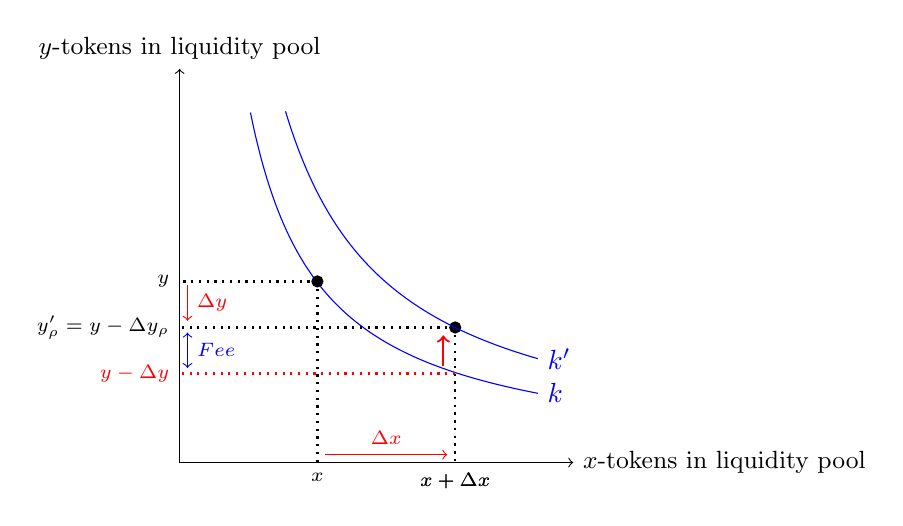
\begin{tikzpicture}[]
    
 	\draw[->] (0,0)--(5,0) node[below,midway]{} node[right] {\small{$x$-tokens in liquidity pool}};	
 	\draw[->] (0,0)--(0,5) node[above,midway,rotate=90]{} node[above] {\small{$y$-tokens in liquidity pool}};

	% before swap
 	\draw[samples = 200, color=blue, scale=1, xshift = 0cm, yshift = 0cm, domain=0.9:4.55, smooth, variable=\x] plot ({\x}, {4/\x}) node[right,color=blue] {$k$} ;    
	\draw[fill=black] (1.75,2.3) circle(2pt);
	\draw[dotted,thick] (1.75,2.3) -- (1.75,0) node[below]{\scriptsize{${x}$}};
	\draw[dotted,thick] (1.75,2.3) -- (0,2.3) node[left]{\scriptsize{$y$}};

	% Delta x
	\uncover<2->{
		\draw[dotted,thick] (3.5,1.13) -- (3.5,0) node[below]{\scriptsize{${x+\Delta x}$}};
		\draw[->, red] (1.85, 0.1) -- (3.4, 0.1) node [midway, above] {\scriptsize{$\Delta x$}};
	}

	% Hypothetical y after (without fees)
	\uncover<3->{
		\draw[dotted,thick, red] (3.5,1.13) -- (0,1.13) node[left, red]{\scriptsize{${y-\Delta y}$}};	
	}
	
	% After swap
	\uncover<4->{
		\draw[dotted,thick] (3.5,1.715) -- (0,1.715) node[left]{\scriptsize{${y'_\rho = y-\Delta y_\rho}$}};	
		\draw[fill=black] (3.5,1.715) circle(2pt);
		\draw[dotted,thick] (3.5,1.715) -- (3.5,0) node[below]{\scriptsize{${x+\Delta x}$}};
	}
	
	\only<4>{
		\draw[-to, thick, red] (3.35, 1.23) -- (3.35,1.615);
	}

	% New k
	\uncover<5->{
	 	\draw[samples = 200, color=blue, scale=1, xshift = 0cm, yshift = 0cm, domain=1.345:4.55, smooth, variable=\x] plot ({\x}, {6/\x}) node[right,color=blue] {$k'$};
	}
	
	% Delta y with fees
	\uncover<6->{
		\draw[->, red] (0.1, 2.25) -- (0.1, 1.8) node [midway, right] {\scriptsize{$\Delta y$}};
	}
	
	% Fees remaining in pool
	\uncover<7->{
		\draw[<->, blue] (0.1, 1.65) -- (0.1, 1.2) node [midway, right] {\scriptsize{$Fee$}};	
	}
\end{tikzpicture}